% ----------------------------------------------------------------
% AMS-LaTeX Paper ************************************************
% **** -----------------------------------------------------------
\documentclass[oneside]{amsart}
\usepackage{graphicx}
\usepackage{color}
\usepackage[letterpaper]{geometry}
\usepackage[colorlinks=false,
            pdfborder={0 0 0},
            pdftitle={CSC469 A2},
            pdfauthor={Daniel Bloemendal},
            pdfsubject={CSC469},
            pdfstartview=FitH,
            pdfmenubar=false,
            pdfdisplaydoctitle=true,
            bookmarks=false]{hyperref}
\usepackage[table]{xcolor}
\usepackage{caption}
\usepackage{subcaption}
\usepackage{mathtools}
\usepackage{listings}
% ----------------------------------------------------------------
\vfuzz2pt % Don't report over-full v-boxes if over-edge is small
\hfuzz2pt % Don't report over-full h-boxes if over-edge is small
% THEOREMS -------------------------------------------------------
\newtheorem{thm}{Theorem}[section]
\newtheorem{cor}[thm]{Corollary}
\newtheorem{lem}[thm]{Lemma}
\newtheorem{prop}[thm]{Proposition}
\theoremstyle{definition}
\newtheorem{defn}[thm]{Definition}
\theoremstyle{remark}
\newtheorem{rem}[thm]{Remark}
\numberwithin{equation}{section}
% MATH -----------------------------------------------------------
\newcommand{\norm}[1]{\left\Vert#1\right\Vert}
\newcommand{\abs}[1]{\left\vert#1\right\vert}
\newcommand{\set}[1]{\left\{#1\right\}}
\newcommand{\Real}{\mathbb R}
\newcommand{\eps}{\varepsilon}
\newcommand{\To}{\longrightarrow}
\newcommand{\BX}{\mathbf{B}(X)}
\newcommand{\A}{\mathcal{A}}
\newcommand{\e}{\mathrm{e}}
\newcommand{\AND}{\wedge}
\newcommand{\OR}{\vee}
\newcommand{\NOT}{\neg}
\newcommand{\IMPLIES}{\to}
\newcommand{\TRUE}{\top}
\newcommand{\FALSE}{\bot}
\newcommand{\EQUALS}{\equiv}
\DeclareMathOperator{\sech}{sech}
% -----------------------------------------------------------------
\begin{document}

\title[CSC469 A2]{CSC469\\ASSIGNMENT 2}
\author{Daniel Bloemendal\\ Simon Scott}
\email{d.bloemendal@utoronto.ca}
\date{November 15, 2013}

% ----------------------------------------------------------------
\begin{titlepage}
\maketitle
\thispagestyle{empty}
\tableofcontents
\end{titlepage}
% ----------------------------------------------------------------

\section{Design}
\subsection{Overview}
Our allocator closely follows the Hoard design discussed in the Emery Berger et al. paper. Memory is
reserved in page sized pieces in the form of superblocks. These superblocks reside in a number of
thread local heaps. The number of these heaps is chosen to be some multiple of the number of
processors on the system. Superblocks are further divided into size classes, which we chose to be
spaced apart by powers of 2. Furthermore, the superblocks are stored into fullness groups based on
how much free space exists in a given superblock. Finally, a global heap is used to prevent
unbounded memory use in certain scenarios. When superblocks reach some emptiness threshold they are
moved to the global heap, and can be acquired by any thread.

\subsection{False sharing avoidance}
The primary goal of the Hoard allocator is to avoid false sharing. Our allocator achieves this by
using thread local heaps. To begin with, the superblocks were carefully chosen to be aligned by
cache line boundaries, as seen in listing \ref{lst:superblock}.
\lstset{language=C, caption={Superblock \& allocation structure}, basicstyle=\footnotesize, label=lst:superblock}
\begin{lstlisting}
// Superblock structure
struct SUPERBLOCK_T {
    heap_t*         heap;
    uint8_t         group;
    int             size_class;
    size_t          block_size;
    size_t          block_count;
    size_t          block_used;
    blockptr_t      next_block;
    blockptr_t      next_free;
    superblock_t*   prev;
    superblock_t*   next;
};

// Allocation structure
struct ALLOCATION_T {
    int type;
    union {
        superblock_t sb;
        largeblock_t lb;
    };
} __attribute__((aligned(ARCH_CACHE_ALIGNMENT)));
\end{lstlisting}

This guarantees that if two threads allocate memory on their own superblocks no false sharing should
occur. However, it should be noted that the process of placing nearly empty superblocks into the
global heap, to be acquired by arbitrary threads, does allow for some limited amount of false
sharing to occur. However, in practice since these superblocks are mostly empty once acquired the
likelihood of false sharing is negligibly small.

\subsection{Unbounded memory use}
The global heap is used as a way to avoid certain scenarios in which unbounded memory usage may
occur. One such scenario is a producer consumer relationship. A producer thread may produce some
object and hand it off to the consumer thread. Once the consumer thread is done with the object, if
there is no way for the producer to reclaim the memory, this can lead to unbounded memory usage.
In our allocator, the consumer would end up relinquishing the superblock after freeing the object,
assuming the superblock is mostly empty afterwards. This successfully mitigates the unbounded memory
problem.

\subsection{Fragmentation}
Superblocks belong to a set of \textit{size classes}, where a superblock of a given size class only
has blocks of the given size. In our implementation these classes are powers of 2. This limits
internal fragmentation to a factor of 2 (Berger et. el., p.2).

\subsection{Cache locality}
Freed blocks are placed in a LIFO. This increase the likelihood of reallocating recently used
memory. This will take advantage of resident TLB entries and other cache effects.

\subsection{Synchronization}
In our implementation, locking is done at thread local heap level. This seems to work very well if
threads mostly allocate and free their own memory only. However, there are some rare scenarios where
significant lock contention occurs. This is illustrated in the Larson benchmark. If threads often
free memory allocated by other threads they prevent other threads from making progress while the
deallocation occurs.

\section{Benchmarking}
\subsection{Hypothesis}
We expected to see very good results in the cache tests. After all, the primary focus of the Hoard
design is to avoid false sharing. Since there were no significantly computationally expensive
algorithms in the code base, we also expected to see reasonably good speed. We also expected to see
less impressive results in the Larson test due to potentially high lock contention.
\subsection{Hardware}
The data was collected in Arch Linux running in VMware Workstation on top of the following hardware
\ref{fig:hardware}.
\begin{figure}[h]
    \caption{vmbox.home hardware}
    \centering
    \begin{tabular}{ll}
        \textbf{Host} & vmbox.home \\
        \hline
        \textbf{CPU} & Intel\textregistered\ Core\texttrademark\ i7-2600K \\
                     & 3.40GHz clock \\
                     & 8MB cache \\
                     & 4 cores \\
                     & 8 threads \\
        \hline
        \textbf{Memory} & 16GB physical \\
                        & 2GB swap \\
        \hline
        \textbf{Kernel} & 3.11.6-1-ARCH x86\_64
    \end{tabular}
    \label{fig:hardware}
\end{figure}

\newpage

\subsection{Data}
As expected, the allocator did well in the cache tests. The figures below show our allocator to be
on par with the Linux system's standard C library.

\begin{figure}[h]
    \caption{Passive false sharing}
    \centering
    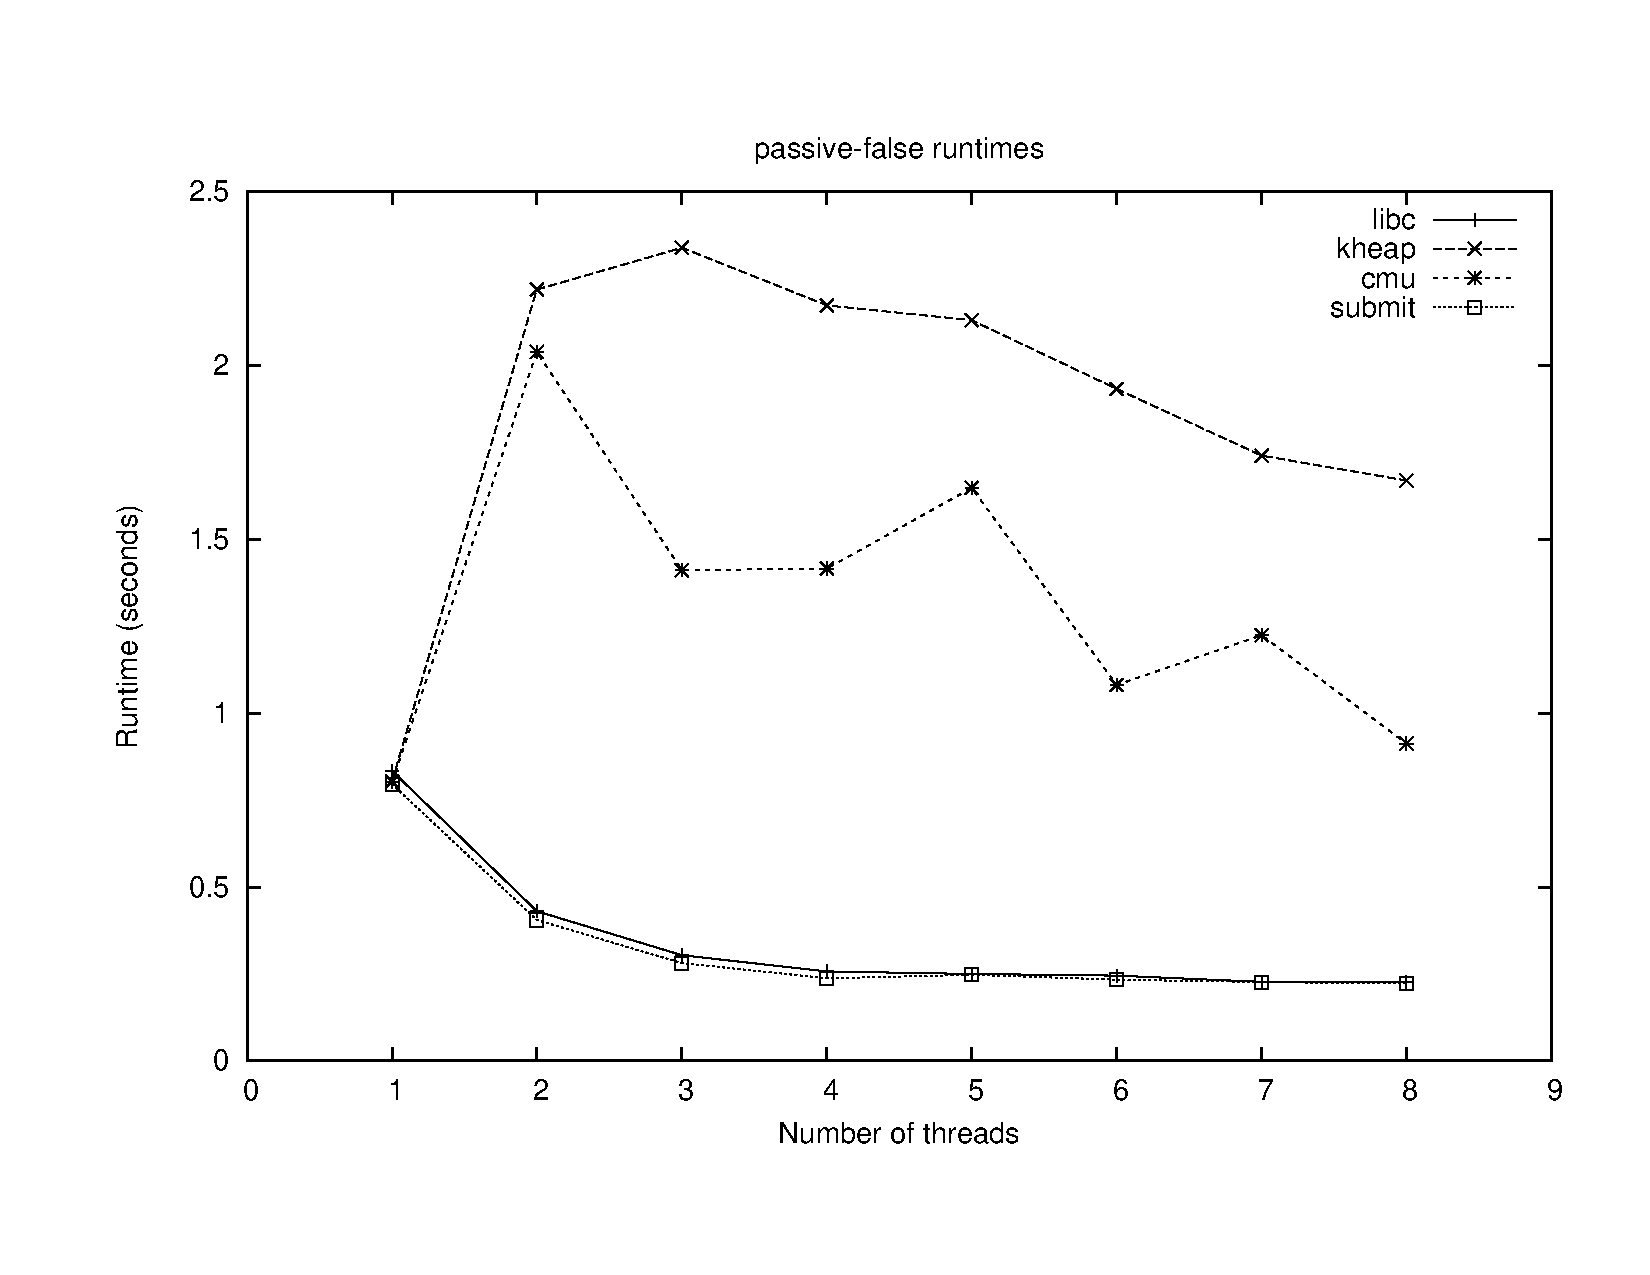
\includegraphics[scale=0.35]{../benchmarks/cache-scratch/cache-scratch.pdf}
    \label{fig:plot}
\end{figure}

\begin{figure}[h]
    \caption{Active false sharing}
    \centering
    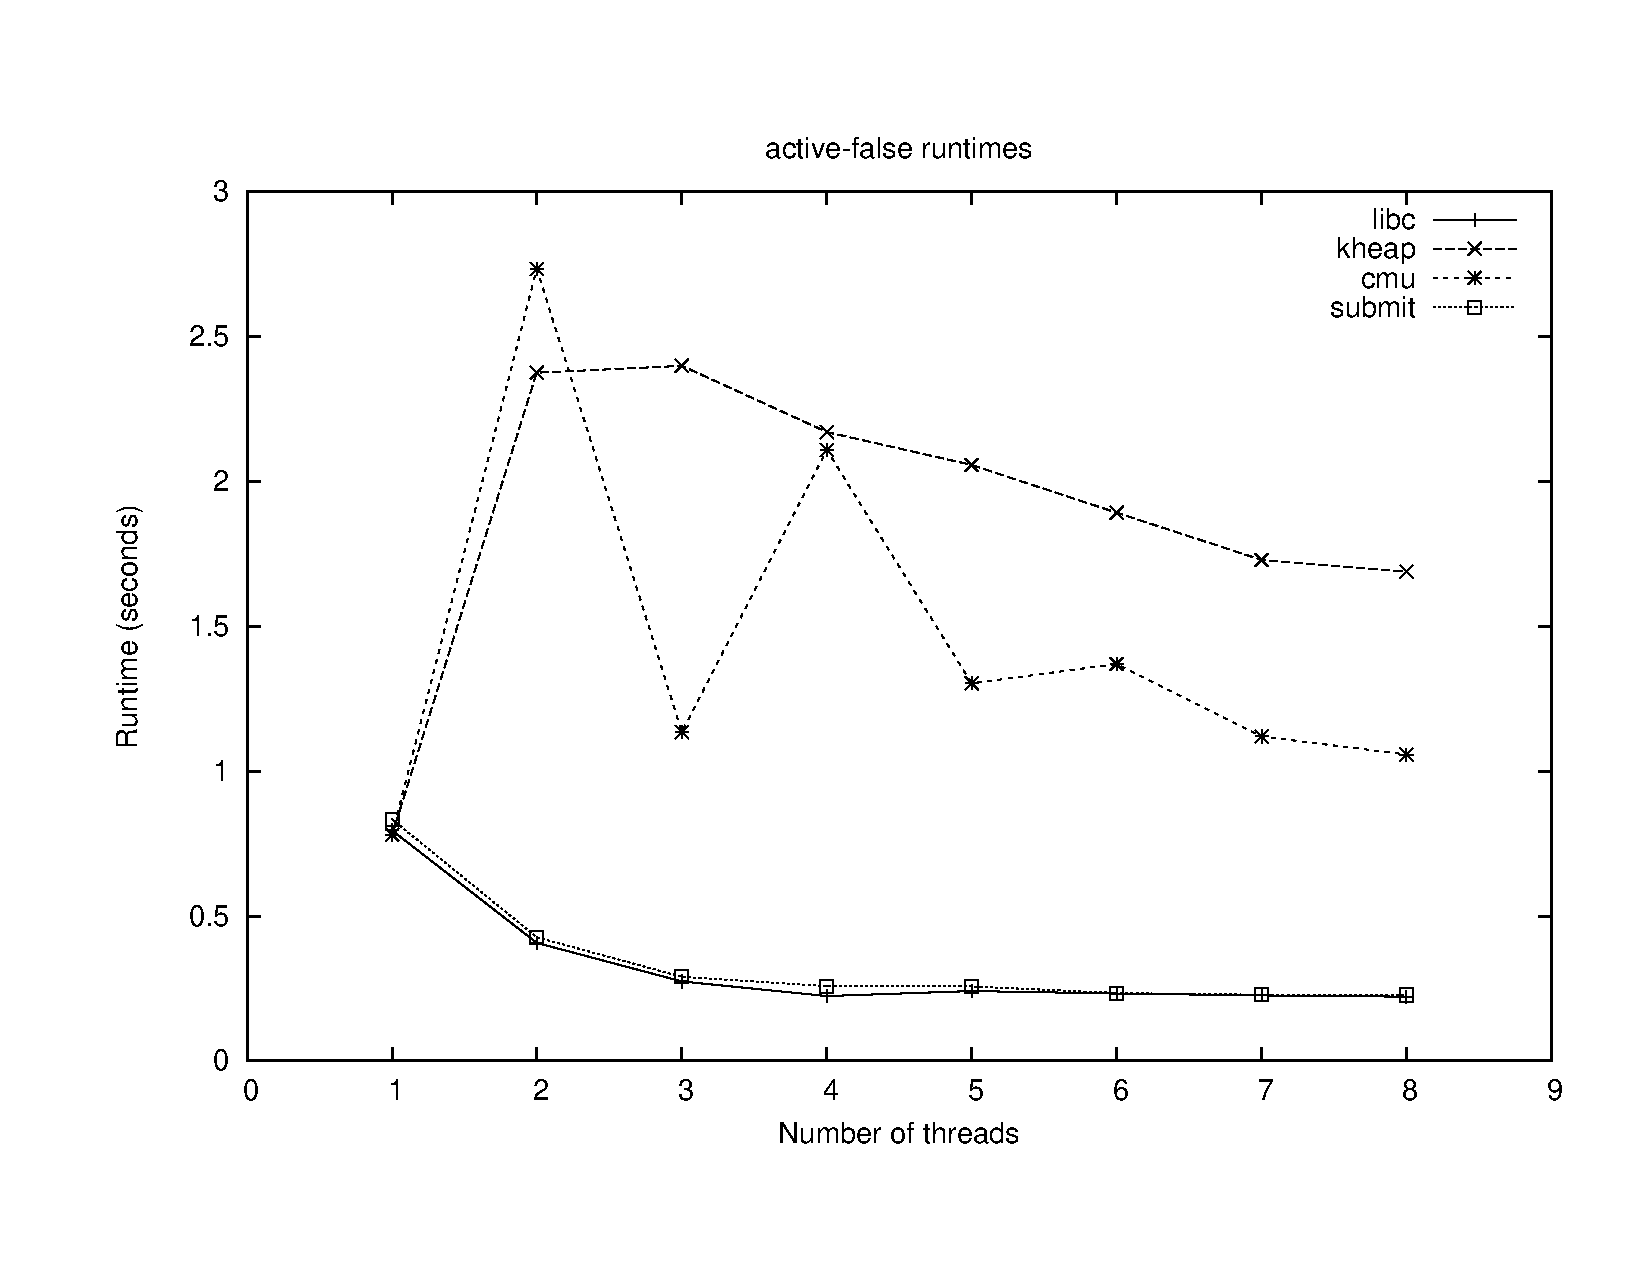
\includegraphics[scale=0.35]{../benchmarks/cache-thrash/cache-thrash.pdf}
    \label{fig:plot}
\end{figure}

\newpage 

The allocator did not do as well in Larson and the Threadtest. There also seems to be some type of
bottleneck at around 8 threads. This is seen in the standard C allocator in the Threadtest
benchmark, but is more pronounced in our allocator in both Larson and the Threadtest. This is most
likely due to the fact that the underlying system is not really an 8 core system but rather a
hyperthreaded 4 core system. Hyperthreading only accelerates context switches.

\begin{figure}[h]
    \caption{Larson}
    \centering
    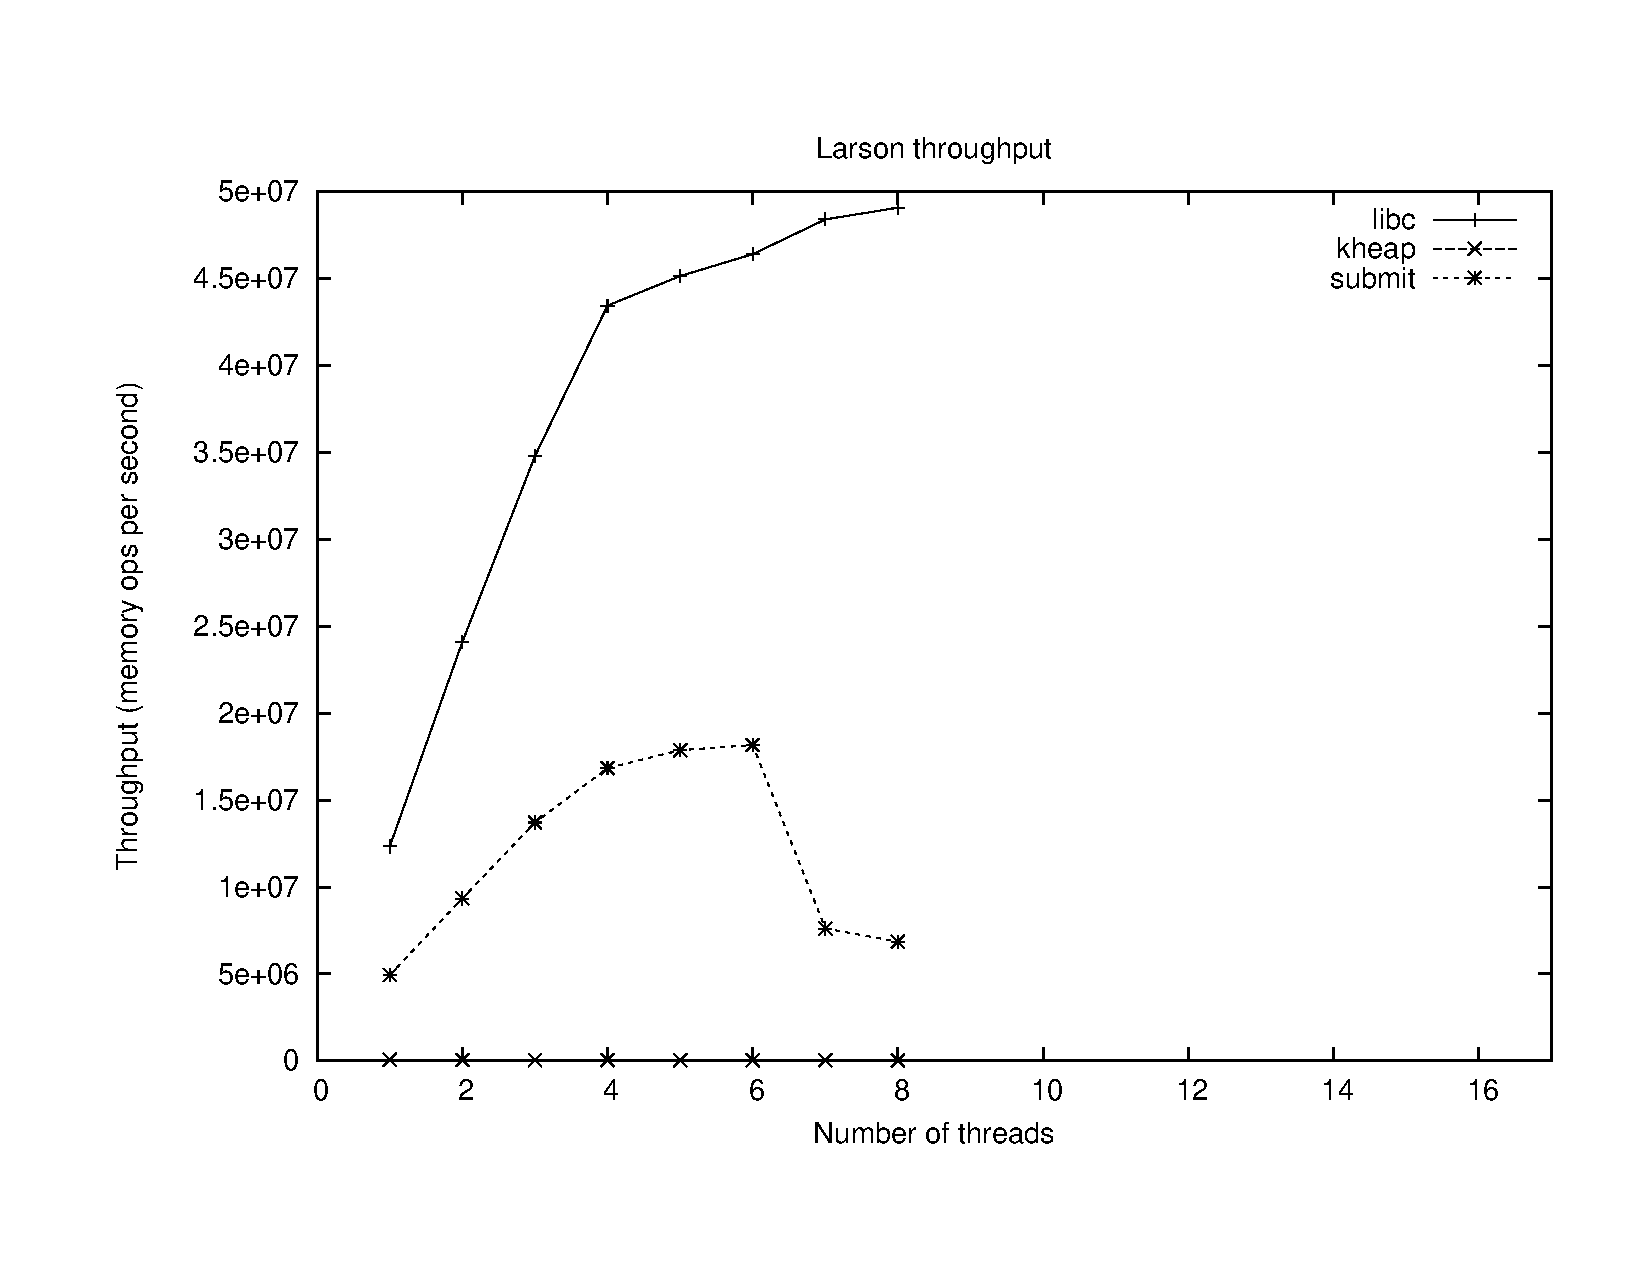
\includegraphics[scale=0.33]{../benchmarks/larson/larson.pdf}
    \label{fig:plot}
\end{figure}

\begin{figure}[h]
    \caption{Threadtest}
    \centering
    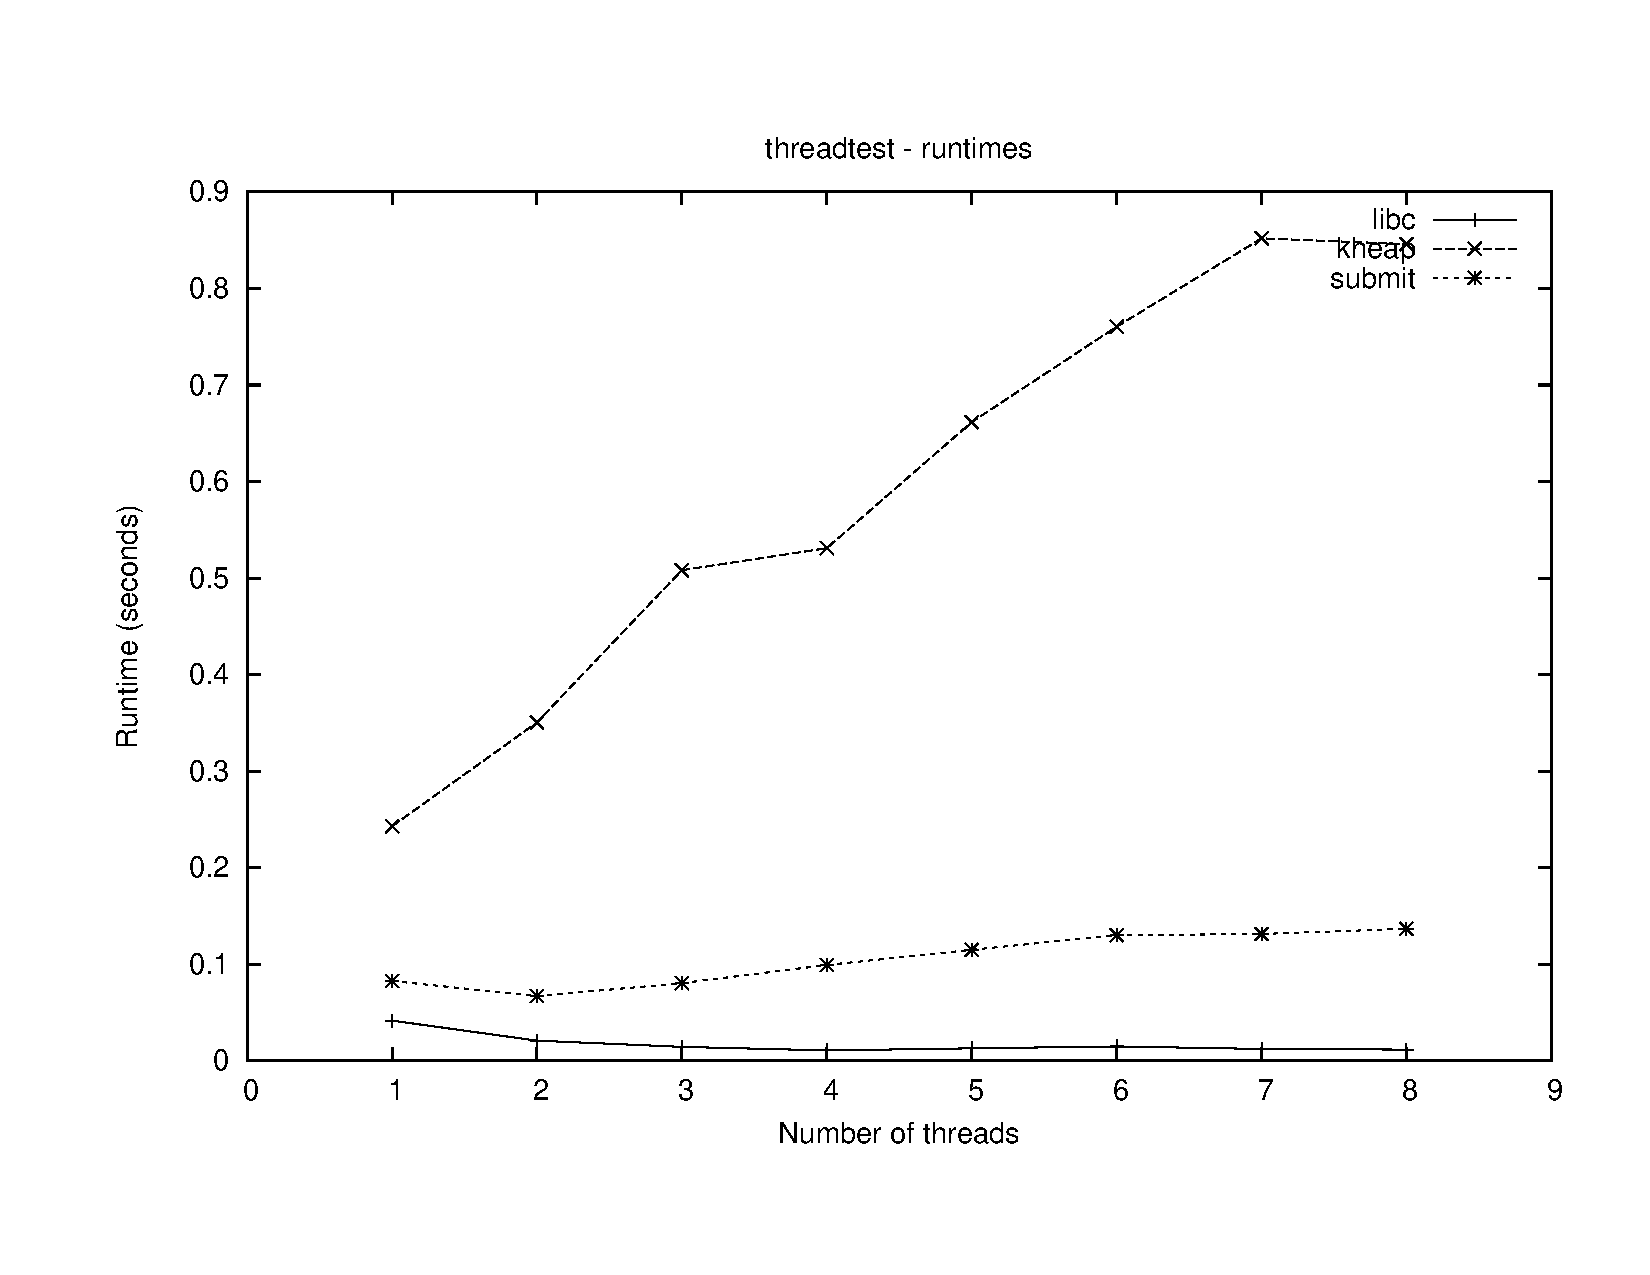
\includegraphics[scale=0.33]{../benchmarks/threadtest/threadtest.pdf}
    \label{fig:plot}
\end{figure}

\subsection{Lock contention analysis}
To confirm our worst fears about the Larson test we decided to perform a more detailed analysis. We
used Intel\textregistered\ VTune\texttrademark\  Amplifier XE 2013 to analyze the lock contention
while the Larson test is running. As mentioned earlier, we expected to see lock contention caused by
the calls to free memory not allocated by the thread doing the freeing.

\begin{figure}[h]
    \caption{VTune}
    \centering
    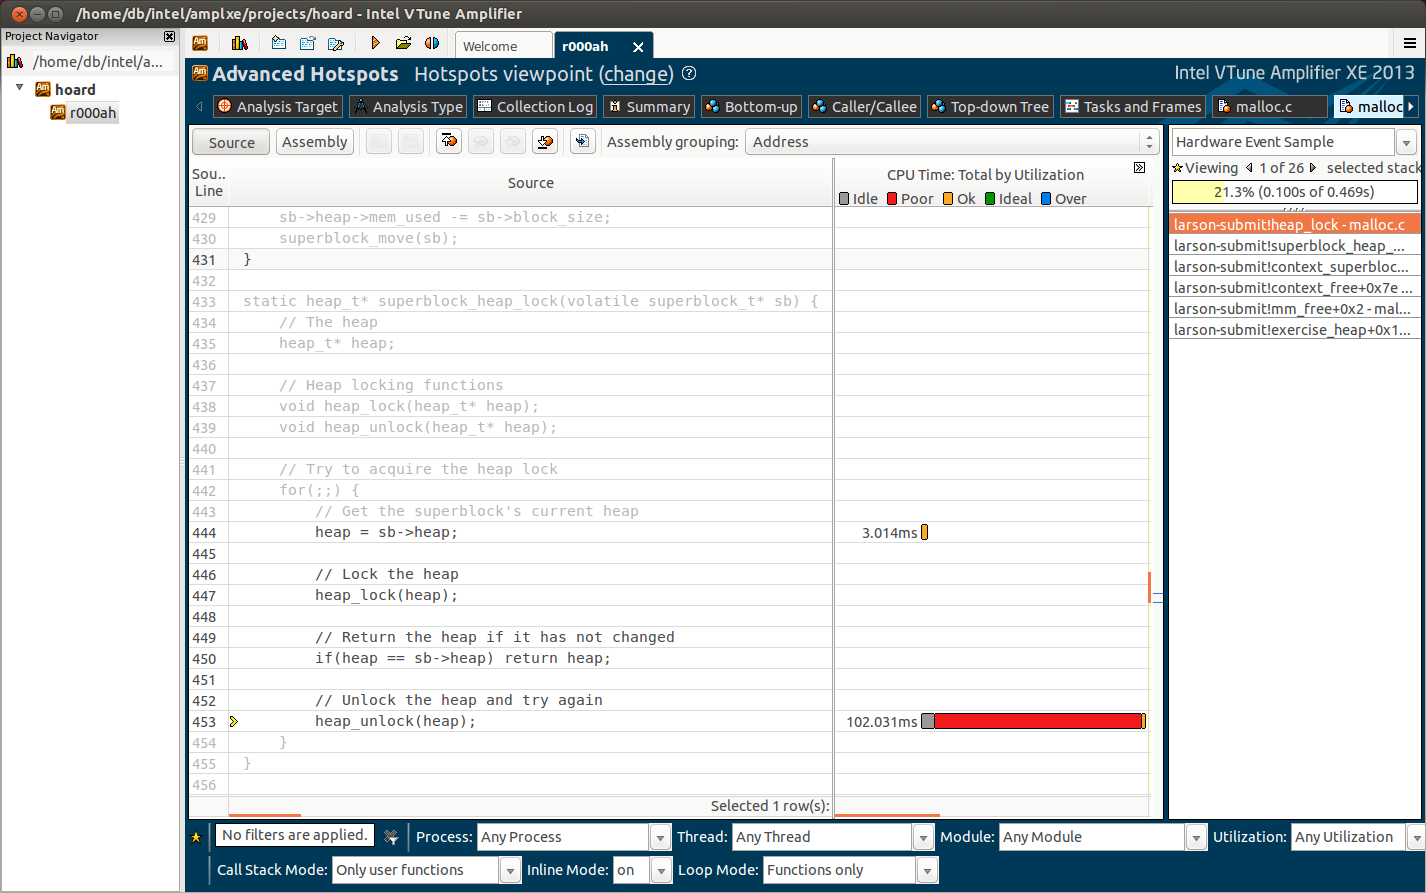
\includegraphics[scale=0.28]{VTune.png}
    \label{fig:plot}
\end{figure}

As expected lock contention is somewhat of a problem during the Larson test.

% ----------------------------------------------------------------
\end{document}
% ----------------------------------------------------------------
